\chapter{绪论}

\section{课题背景}

将跨越不同行业、组织、价值链等边界的服务进行深度融合和模式创新,为用户提供多维度、高质量、富价值的跨界服务,成为现代服务业发
展的重要创新途径。然而,目前针对跨界服务本质规律认知、跨界服务融   
合理论、工程设计方法与运行载体等方面仍然缺少系统研究,缺少充分理
论指导的跨界服务融合实践呈现一定的盲目性,极大影响我国现代服务业
的创新发展。

依托以互联网为代表的信息技术的高速发展,我国社会当前正处在由传统服务业向现
代服务业全面升级的重要历史进程中。充分利用和结合现代先进的信息技术,提供信息和
知识更加密集、附加值更高的服务是现代服务业的基本要求。互联网作为现代信息服务的
载体,从早期简单的门户网站、搜索引擎,发展到社交网站、即时通信,再到移动搜索、LBS
等移动互联网应用的风靡,在产业规模持续扩大的同时,也不断向各行各业渗透,从早期
的传媒、游戏等行业,到娱乐、零售行业,再到金融、教育和医疗等行业,影响范围还在不
断继续扩大\cite{王晓玲2015我国现代服务业借力}。由此可见,未来服务的基础形态一定是基于互联网的,各行业通过互联网来
提供他们的服务是大势所趋。

\begin{figure}[htbp]
    \centering
    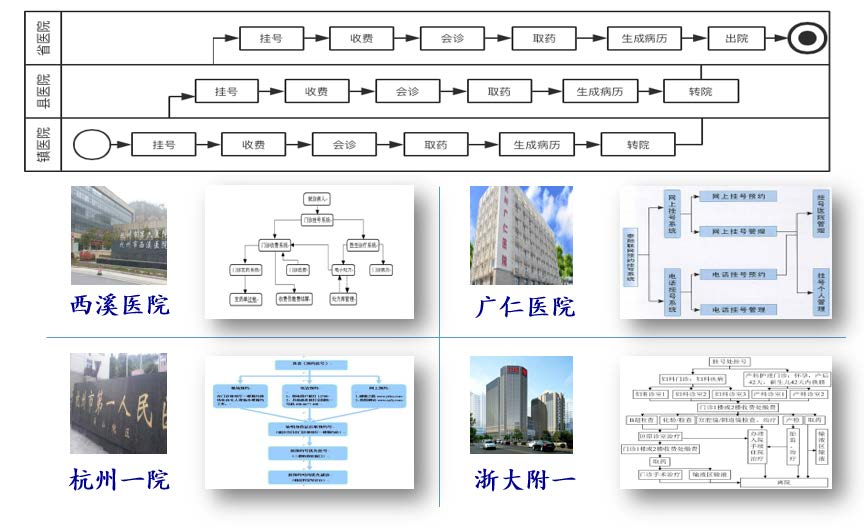
\includegraphics[scale=1]{./images/hospitalRunningModel.jpg}
    \caption{传统医院经营模式图}
    \label{fig:example}
  \end{figure}

早期的基于网络的应用服务通常构建于一组相互联系的Web Service 之上。根据W3C
的定义,Web Service 是指用于支持网络内机器之间互操作的软件系统,它通常包含一个机
器可处理的接口描述(一般是WSDL),其它系统按照其接口描述通过SOAP 消息与它进行
交互\cite{verborgh2018web}。Web Service 包含一系列标准化的规范和技术用以支持基于Web 的应用的集成,包
括XML, SOAP, WSDL 和UDDI 等。

Web Service 在早期许多大型企业级软件应用中使用广泛,但由于其相关标准和技术过
于复杂等原因,在如今的新兴互联网应用中已经很少使用了。目前Web API,作为一种更
加灵活和轻量级的解决方案,摒弃了WS 系列的相关复杂标准,得到了广泛的应用\cite{zaveri2017smartapi}。


